

\section{Classical DP}

\begin{frame}
  \begin{center}
    {\bf Part II -- Classical DP Problems}
  \end{center}
\end{frame}

\begin{frame}{Classical DP Problems}

  There are some classical problems that have well known DP solutions:
  \bigskip

  \begin{itemize}
    \item Max sum;
    \item Max sum 2D;
    \item Longest Increasing Subsequence;
    \item Knapsack Problem;
    \item Coin Change;
  \end{itemize}
  \bigskip

  We will show some examples from each category so you can have a better understanding of the DP philosophy.\bigskip

  {\bf After each problem is explained, try to find the DP table, and the transition function}.
\end{frame}

\subsection{Max Sum}

\begin{frame}[fragile]{The 1D Range Sum Problem}

  Consider an array $A$ containing $N$ integers. We want to find the indexes $i,j, (0 \leq i < j \leq N-1)$ that {\bf maximize} the sum from $A_i$ to $A_j$ ($\sum_{k=i}^{j} A_k$).
  \bigskip

  Example:
\begin{verbatim}
Array A = 1, -3, 20, -2, -5, 10, 5, -4, 6, 47, -30, -3
  Total = 42
RangeSum=        20, -2, -5, 10, 5, -4, 6, 47
  Total = 77
\end{verbatim}
\bigskip

How do you solve this problem?
\end{frame}

\begin{frame}[fragile]{The 1D Range Sum Problem}{Complete Search}
  \begin{block}{    Calculate the range sum for every possible pair $(i,j)$.}

{\smaller
\begin{verbatim}
int minindex, maxindex;
int maxsum = 0;
for (int i = 0; i < n; i++)             // Loop 1
   for (int j = 0; i < n; j++)          // Loop 2
      int sum = 0;
      for (int k = i; k < j+1; k++)     // Loop 3
         sum += k;
      if sum > maxsum:
         maxsum = sum;
         minindex = i; maxindex = j;
\end{verbatim}
}
  \end{block}

  Because of three loops, this approach is $O(n^3)$. For large values of $N$ ($N > 10.000$), this is a bad idea.
\end{frame}

\begin{frame}[fragile]{The 1D Range Sum Problem}{DP Sum Table}
  Note that {\bf sum(i,j) = sum(0,j) - sum(0,i-1)}.\medskip

  Using this fact, we can create a sum table (ST) to calculate the result faster:

  \begin{block}{Using Sum Table -- $O(n^2)$}
{\smaller
\begin{verbatim}
int[] ST; int maxsum = 0; int sum_s = 0; int sum_e = 0; ST[0] = 0;

for (int i = 1; i < N+1; i++) { ST[i] = ST[i-1] + A[i]; } // preprocessing;

for (int i = 1; i < N+1; i++)
  for (int j = i; j < N+1; j++)
    if (ST[j] - ST[i-1] > maxsum) {
      maxsum = ST[j] - ST[i-1];
      sum_s = i; sum_e = j;
    }
\end{verbatim}
}
  \end{block}
\end{frame}

\begin{frame}[fragile]{The 1D Range Sum Problem}{DP Sum Table Simulation}

  Let's visualize how the DP sum table transforms the problem:

{\smaller
\begin{verbatim}
i  =      1,  2,  3,  4,  5,  6,  7,  8,  9, 10, 11, 12
A  =      1, -3, 20, -2, -5, 10,  5, -4,  6, 47,-30, -3
ST = [0], 1, -2, 18, 16, 11, 21, 26, 22, 28, 75, 45, 42

i, j  | ST[j] - ST[i-1] | Total Sum
===================================
1, 12 | 42    - 0       | 42
3, 10 | 75    - (-2)    | 77
6, 8  | 22    - 11      | 11
===================================
\end{verbatim}
}
\bigskip

Can we do even better?
\end{frame}

\begin{frame}[fragile]{The 1D Range Sum Problem}
  {Kadane's Greedy Algorithm -- $O(n)$ mix of Sum Table and Greedy Approach}

  \begin{block}{}
      {\smaller
\begin{verbatim}
A[] = { 4, -5, 4, -3, 4, 4, -4, 4, -5}; // Example
int sum = 0, ans = 0;
for (i in 0:n):
   sum += A[i], ans = max(ans, sum)     // Add to running total
   if (sum < 0) sum = 0;                // If total is negative
                                        // reset the sum;
\end{verbatim}
      }
  \end{block}

\begin{itemize}
\item Basic idea: it is always better to increase the sum,
unless a very large negative sum appears.
\item In that case, it is better to start from zero after the negative sum.
\end{itemize}
\begin{verbatim}
    A  :  4 | -5 | 4 -3  4  4 -4  4 | -5
    Sum:  4 |  0 | 4  1  5  9  5  9 |  4
    ans:  4 |  4 | 4  4  5  9  9  9 |  9
\end{verbatim}
\end{frame}

\subsection{Maximum Sum -- 2D}
\begin{frame}
  \frametitle{Maximum Range Sum -- Now in 2D!}
  \begin{block}{Problem Summary}
    Given an array of positive and negative numbers, find the
    subarray with maximum sum.
  \end{block}
  \begin{center}
    \begin{tabular}{|cccc|}
      \hline
      0 & -2 & -7 & 0\\
      9 & 2 & -6 & 2\\
      -4 & 1 & -4 & 1\\
      -1 & 8 & 0 & -2\\
      \hline
    \end{tabular}
  \end{center}
  \bigskip

  This is the same problem as the previous one, but the second dimention adds some interesting complications.\bigskip

  {\bf QUIZ:}
  \begin{itemize}
    \item What is the cost of a complete search in this case?
    \item How would you write a DP (table and loop)?
  \end{itemize}
\end{frame}

\begin{frame}[fragile]{Maximum Range Sum 2D}{Complete Search}

\begin{block}{}
  The complete search approach needs 6 loops (2 for horizontal axis, 2 for vertical axis, 2 for calculating the sum). So the total complexity is O($n^6$).
\end{block}

\begin{block}{}
{\smaller
\begin{verbatim}
minvalue = -MIN_INT
for i in (0:n):
   for j in (0:n):
      for k in (i:n):
         for l in (j:n):
         sum = 0
         for a in (i:k):
            for b in (j:l):
               sum += A[a,b]
         if sum > minvalue:
            minvalue = sum
\end{verbatim}
}
\end{block}
\end{frame}

\begin{frame}[fragile]{Maximum Range Sum 2D}{Using the Sum Table}

We can use the Sum Table idea from 1D, but be careful about the {\bf Principle of Inclusion-Exclusion}. We subtract the partial sum of two axis, and add back the intersection of that sum.
\bigskip

\begin{columns}
  \column{0.5\textwidth}
  \hfill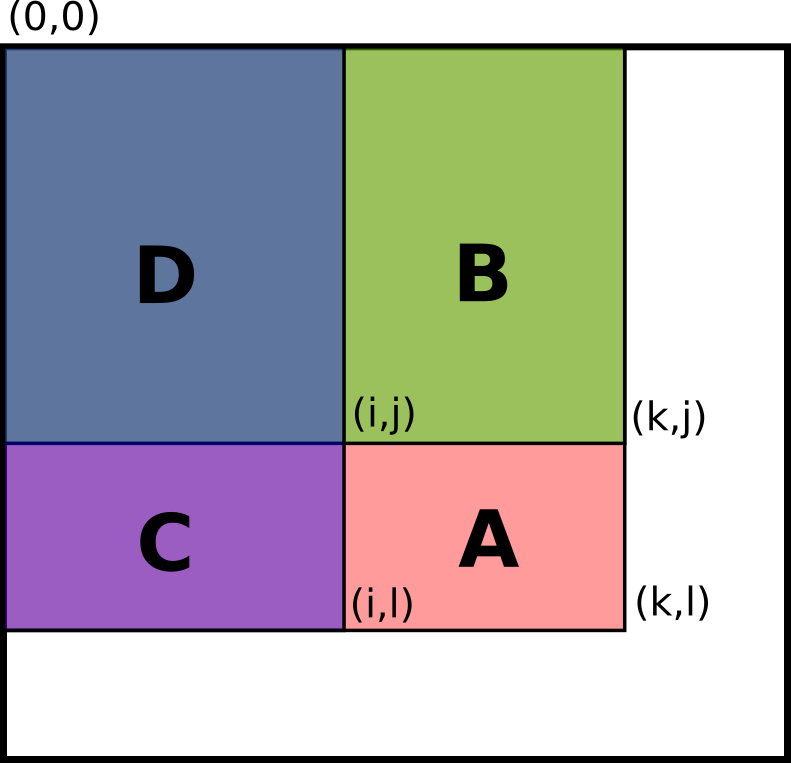
\includegraphics[width=.6\textwidth]{img/inclusion_exclusion}
  \column{0.5\textwidth}
  $A = ABCD - BD - CD + D$
\end{columns}

\end{frame}

\begin{frame}[fragile]{Maximum Range Sum 2D}{2D Sum Table Pseudocode}
\begin{block}{}
{\smaller
\begin{verbatim}
for i in (0:n):                      // Precalculation: Creating ST
   for j in (0:n):
       ST[i][j] = A[i][j]                            // A[i][j] is the input
       if (i > 0) ST[i][j] += ST[i-1][j]
       if (j > 0) ST[i][j] += ST[i][j-1]
       if (i > 0 && j > 0) ST[i][j] -= ST[i-1][j-1]  // Avoid double count

for i,j in (0:n)(0:n):
   for k,l in (i:n)(j:n):
      sum = ST[k][l]                         // Total Sum (0,0)->(k,l)
      if (i > 0) sum -= ST[i-1][l];          // Remove (0,0)->(i-1,l)
      if (j > 0) sum -= ST[k][j-1];          // Remove (0,0)->(k,j-1)
      if (i > 0 && j > 0) sum += A[i-1][j-1] // Add back double remove
      maxsum = max(sum,maxsum)
\end{verbatim}
}
\end{block}

\end{frame}

\subsection{Longest Increasing Subsequence}

\begin{frame}[fragile]{Problem 3: Longest Increasing Subsequence}{Problem Definition}
  \begin{block}{}
    Given a sequence $A$ of integers, find the longest subsequence $S \in A$ where $S_i < S_{i+1} < S_{i+2} < \ldots$.
  \end{block}
  \bigskip

  Example:
\begin{verbatim}
A   = [-7, 10, 9, 2, 3, 8, 8, 1]
S_1 = [-7,        2, 3, 8]          // size 4 -- LIS
S_2 = [-7,     9]                   // size 2
\end{verbatim}
\bigskip

Note that because the subsequence is {\bf not contiguous}, this problem is more difficult than Range Sum.
\bigskip

{\bf QUIZ}: What is the \alert{Complete Search} and \alert{DP approach} (Table and Loop) for this problem?
\end{frame}

\begin{frame}[fragile]
  \frametitle{Complete Search for LIS}

  As other "find the subset" problems, the complete search of LIS can be done by testing all binary strings of size "n". This costs $O(2^n)$.
  \smallskip

  \begin{block}{}
    {\smaller
\begin{verbatim}
// Complete Subset Search using bitmasks
vector<int> S_max; int max_len = 0;// Final Result

for (int i = 0; i < (1<<n); i++) {                // Loop all bitstrings
  vector<int> S; int min = -99999; int len = 0;
  for (int j = 0; j < n; j++) {                   // Creat subset from bitstring
    if ((1<<j)&i) {                               // Add j to subset
      if (A[j] > min) {                           // Test if subset is increasing
        S.push_back(A[j]);
        min = A[j]; len ++;
      } else { break; }                           // Subset not increasing
  } }
  if (len > max_len) { max_len = len; S_max = S; }// Found a longer subset
} }
\end{verbatim}
    }
  \end{block}
\end{frame}

\begin{frame}{DP for Longest Increasing Subsequence}
  As usual, to prepare a DP we decide the {\bf Table} and {\bf Transition}.

  \begin{block}{Transition}
    Loop each element A[i], and choose:
    \begin{itemize}
      \item Check A[0] to A[i-1], see if A[i] can enter an existing LIS
      \item If not, A[i] is the beginning of a new LIS
    \end{itemize}
  \end{block}

  \begin{exampleblock}{Tables}
    \begin{itemize}
      \item {\bf A[i]}: Has the value of the number;
      \item {\bf Parent[i]}: Has the index of the previous number in the LIS;
      \item {\bf LIS[i]}: Size of the longest LIS that this number is a member;
    \end{itemize}
  \end{exampleblock}
\end{frame}

\begin{frame}[fragile]{DP for Longest Increasing Subsequence}{Example}
\begin{verbatim}
  A      = [  0, 10, 9,  0, 3, 8, 8, 1 ]
  parent = [ -1,  0, 0, -1, 3, 4, 4, 3 ]
  LIS    = [  1,  2, 2,  1, 2, 3, 3, 2 ]
\end{verbatim}

\begin{block}{Pseudocode (O($n^2$))}
\begin{verbatim}
LIS[0:n] = 1
parent[0:n] = -1
for i in (1 to n):
   for j in (0 to i): // Try to add to longest LIS
      if (LIS[j] >= LIS[i]) && (A[j] < A[i]):
         LIS[i] = LIS[j] + 1
         parent[i] = j
\end{verbatim}
\end{block}

There is a faster $O(n\log k)$ approach that uses greedy and binary search.
\end{frame}


\subsection{Knapsack problem}
\begin{frame}[fragile]{Classic DP: The 0-1 Knapsack Problem}

  In the 0-1 Knapsack problem (also known as "subset sum"), there is a set $A$ of items with size $S$ and value $V$.\bigskip

  You have to select a subset $X \subseteq A$ where the sum of sizes $ \leq M$, and the sum of values is maximum.\bigskip

\begin{verbatim}
Input:
  A<S,V> = [ (10, 100), (4, 70), (6, 50), (12, 10)]
  M = 12

Solution:
  [ (4,70), (6,50) ]
\end{verbatim}\bigskip

{\bf QUIZ}: What is the complete search and the DP (Table, Transition)?\\
{\bf Hint:} This problem is similar to the "Wedding Problem".
\end{frame}

\begin{frame}[fragile]{0-1 Knapsack -- Complete Search}
  The solution to the complete search is to test all subsets of A. This approach, as you know, takes $O(2^n)$.\bigskip

  This time, instead of a binary string, we will test all combinations using {\bf recursion}.

  \begin{block}{Complete Search Recursive Solution}
    Recursive function: \emph{value(id,size)}, where \emph{id} is the item we want to add, and \emph{size} is the size remaining after we add id in the backpack.\medskip

\begin{verbatim}
value(id,size):
   if (size < 0): return 0   # bag is full
   if (id == n):  return 0   # checked all items
   # either add the item, or do not add the item
   return max(value(id+1,size),
              V[id] + value(id+1, size - S[id]))
\end{verbatim}
  \end{block}
\end{frame}

\begin{frame}[fragile]{0-1 Knapsack -- Top-down DP}
  From the recursive function, it is very easy to use a DP table as memory for value(id, size).\medskip

    {\bf Be careful}: The DP table size (and the execution time) is $|A|\times M$. If $M$ is too big ($>> 10^6$), you might get TLE or MLE.
\begin{verbatim}
A<S,V> = [ (10, 100), (4, 70), (6, 50), (12, 10)]
M = 12

value(i,size):
\end{verbatim}

  \begin{center}
  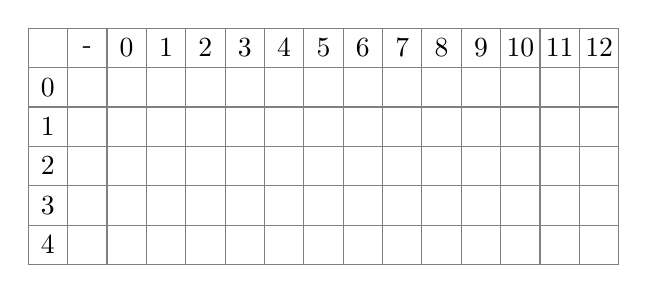
\begin{tikzpicture}
  \draw[step=0.5cm,color=gray] (0,0) grid (7.5,3);
  %% Row 0
  \node at (.75,2.75) {-};
  \node at (1.25,2.75) {0};
  \node at (1.75,2.75) {1};
  \node at (2.25,2.75) {2};
  \node at (2.75,2.75) {3};
  \node at (3.25,2.75) {4};
  \node at (3.75,2.75) {5};
  \node at (4.25,2.75) {6};
  \node at (4.75,2.75) {7};
  \node at (5.25,2.75) {8};
  \node at (5.75,2.75) {9};
  \node at (6.25,2.75) {10};
  \node at (6.75,2.75) {11};
  \node at (7.25,2.75) {12};
  %% Column 0
  \node at (.25,2.25) {0};
  \node at (.25,1.75) {1};
  \node at (.25,1.25) {2};
  \node at (.25,.75) {3};
  \node at (.25,.25) {4};
  \end{tikzpicture}\bigskip
  \end{center}


\end{frame}

\subsection{Coin Change}
\begin{frame}[fragile]{Classical DP -- The Coin Change Problem (CC)}{Problem Summary}
  You are given a target value $V$, and a set $A$ of coin sizes. You have to find the smallest sequence of coins (with repetition) that adds to $V$.
  \bigskip

Example:
\begin{verbatim}
V = 7
A = {1, 3, 4, 5}
  S_0 = { 1, 1, 1, 1, 3}
  S_1 = { 5, 1, 1}
  S_2 = { 3, 3, 1}
  S_3 = { 4, 3}
\end{verbatim}

The best solution is $S_3$.\bigskip

{\bf QUIZ}:
\begin{itemize}
  \item How do you solve this by complete search?
  \item What is the DP Table and Transition?
\end{itemize}
\end{frame}

\begin{frame}[fragile]
  \frametitle{Complete Search for Coin Change}

  We can build a recursive search using the following recurrence on the number of coins $N$ necessary for a given value $V$:
  \[N(V) = 1 + N(V-\text{ size of coin})\]

  \begin{block}{Recursive Complete Search}
    {\smaller
\begin{verbatim}
coins(V):                           // Number of coins for value V:
   if V == 0: return 0              // 0 coins for value 0
   if V < 0:  return MAX_INT        // Can't satisfy for this value
   min = INF                        // Minimum number of coins
   for i in (coins):                // Test each coin
      t = 1 + change(value - A[i])
      if (t < min): min = t
   return t
\end{verbatim}
  }
  \end{block}
\end{frame}

\begin{frame}[fragile]{DP for Coin Change}
  \begin{itemize}
    \item Implementing a Top-down DP should be easy for you now;
    \item Let's make a Bottom-UP DP for practice.
    \item For Bottom-UP DP, it is easier to use a table indexed on COINS
  \end{itemize}

\begin{block}{Bottom-UP DP}
  {\smaller
\begin{verbatim}
boolean DP[c][v] = FALSE;     // Can we reach v with c coins?

i = 0; DP[0][0] = TRUE;       // Start condition
while (TRUE):
  i+=1; possible = FALSE      // Start the loop
  for j = 0 to V:
    if (DP[i-1][j]):          // For each reachable value of V
      possible = TRUE         // We can continue
      if (j == V): return c-1 // Found a solution, go back!
      for k in (coins):       // update all coins
        DP[i][j+k] = TRUE     // Mark new reachable values
  if (!possible): return -1   // No solution found
\end{verbatim}}
\end{block}
\end{frame}

\begin{frame}[fragile]{DP for Coin Change}{Simulation}
\begin{verbatim}
V = 7
A = {1, 3, 4, 5}
\end{verbatim}

\begin{center}
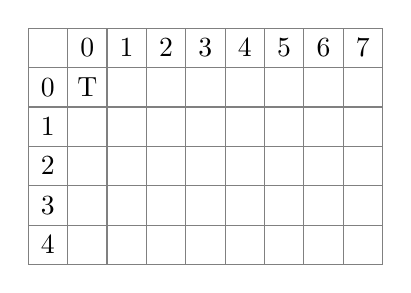
\begin{tikzpicture}
\draw[step=0.5cm,color=gray] (0,0) grid (4.5,3);
%% Row 0
\node at (.75,2.75) {0};
\node at (1.25,2.75) {1};
\node at (1.75,2.75) {2};
\node at (2.25,2.75) {3};
\node at (2.75,2.75) {4};
\node at (3.25,2.75) {5};
\node at (3.75,2.75) {6};
\node at (4.25,2.75) {7};
%% Column 0
\node at (.25,2.25) {0};
\node at (.25,1.75) {1};
\node at (.25,1.25) {2};
\node at (.25,.75) {3};
\node at (.25,.25) {4};
%% Starting Value
\node at (.75,2.25) {T};
\end{tikzpicture}\bigskip
\end{center}
\bigskip

It is interesting to note that the calculation of row $i$ depends only on row $i-1$. Using this information, you can implement the program with a much smaller table.

\end{frame}

%\subsection{Travelling Salesman Problem}
%\begin{frame}
%  \frametitle{Classical DP -- Travelling Salesman Problem}
%
%  We will talk about TSP with DP Next Class!
%\end{frame}

%%%%%%%%%%%%%%%%%%%%%%%%%%%%%%%
% Travelling Salesman Problem (bitmask again)
%% Travelling Salesman Problem (TSP)
% State: tsp(pos,bitmask)
% Transition:
%   Each visited city is a bit in the bitmask
%   - if every city has been visited: tsp(pos, 2^n -1) = dist[pos][0] (back to the start with 0 cities)
%   - Else, try visiting unvisited cities one by one
%   - tsp(pos,bitmask) = min (dist[pos][nxt] + tsp(nxt,bitmask|1<<nt))) for every nxt != pos,
%                                                                           and nxt not visited
%                                                                           bitmask & 1<<nxt == 0
